\clearpage
\begin{examplebox}
\textbf{\textcolor{CExample}{例1：求点与直线的镜像（入门）}}
\begin{center}
\begin{minipage}{\linewidth}\centering
\begin{tikzpicture}[x=1.35cm,y=1.35cm,>=stealth,font=\small,line cap=round,line join=round]
\draw[->,gray!75] (-3.3,0)--(3.46,0) node[right=3pt]{$x$};
\draw[->,gray!75] (0,-3.3)--(0,3.46) node[above=3pt]{$y$};
\node at (-.5,.7) {$O$};
\draw[gray,dashed] (-3.3,-3.3)--(3.3,3.3) node[above left=3pt]{$y=x$};

\draw[teal,very thick] (-2,-3)--(1,3);
\draw[blue,very thick] (-3,-2)--(3,1);
\draw[orange!80!black,densely dotted,thick] (1,3)--(3,1);
\fill[teal] (1,3) circle(2pt) node[above=6pt]{$P(1,3)$};
\fill[blue] (3,1) circle(2pt) node[below=6pt]{$P'(3,1)$};

\end{tikzpicture}\par\smallskip
{\small \textcolor{teal}{\rule[.5ex]{1em}{.8pt}\ $y=2x+1$}\qquad\textcolor{blue}{\rule[.5ex]{1em}{.8pt}\ $y=(x-1)/2$}}\par
{\small 两条直线互为镜像，斜率分别为 $2$ 与 $1/2$。}\par\smallskip
\end{minipage}
\end{center}


求点 $P(1,3)$ 与直线 $y=2x+1$ 关于 $y=x$ 的镜像。

\textbf{解：}点交换坐标得 $P'(3,1)$。直线交换变量得 $x=2y+1$，移项得 $2y=x-1$，所以 $\boxed{y=(x-1)/2}$。原斜率为 $2$，镜像为 $1/2$，不是 $-1/2$。
\end{examplebox}
\clearpage
\begin{examplebox}
\textbf{\textcolor{CExample}{例2：求指数函数的反函数（基础）}}
\begin{center}
\begin{minipage}{\linewidth}\centering
\begin{tikzpicture}[x=1.35cm,y=1.35cm,>=stealth,font=\small,line cap=round,line join=round]
\draw[->,gray!75] (-3.3,0)--(3.46,0) node[right=3pt]{$x$};
\draw[->,gray!75] (0,-3.3)--(0,3.46) node[above=3pt]{$y$};
\node at (-.3,.4) {$O$};
\draw[gray,dashed] (-3.3,-3.3)--(3.3,3.3) node[above left=3pt]{$y=x$};

\draw[teal,very thick,domain=-3:1.65,samples=120] plot(\x,{2^\x});
\draw[blue,very thick,domain=-3:1.65,samples=120] plot({2^\x},\x);
\draw[orange!80!black,densely dotted] (1,2)--(2,1);
\fill[teal] (0,1) circle(2pt) node[left=4pt]{$(0,1)$};
\fill[blue] (1,0) circle(2pt) node[below right=8pt]{$(1,0)$};
\fill[teal] (1,2) circle(2pt) node[above left=4pt]{$(1,2)$};
\fill[blue] (2,1) circle(2pt) node[below right=4pt]{$(2,1)$};

\end{tikzpicture}\par\smallskip
{\small \textcolor{teal}{\rule[.5ex]{1em}{.8pt}\ $y=2^x$}\qquad\textcolor{blue}{\rule[.5ex]{1em}{.8pt}\ $y=\log_2x$}}\par
{\small 原函数与反函数的对应点交换横纵坐标。}\par\smallskip
\end{minipage}
\end{center}


求 $f(x)=2^x$ 的反函数及定义域。

\textbf{解：}原定义域为 $\mathbb R$，值域为 $(0,+\infty)$，且严格递增。交换得 $x=2^y$，根据对数定义 $y=\log_2 x$，故 $\boxed{f^{-1}(x)=\log_2 x,\ x>0}$。验证：$\log_2(2^x)=x$，$2^{\log_2 x}=x$（$x>0$）。
\end{examplebox}
\clearpage
\begin{examplebox}
\textbf{\textcolor{CExample}{例3：求二次函数的反函数（定义域）}}
\begin{center}
\begin{minipage}{\linewidth}\centering
\begin{tikzpicture}[x=1.65cm,y=1.65cm,>=stealth,font=\small,line cap=round,line join=round]
\draw[->,gray!75] (-0.35,0)--(4.96,0) node[right=3pt]{$x$};
\draw[->,gray!75] (0,-0.35)--(0,4.96) node[above=3pt]{$y$};
\node at (-.3,.4) {$O$};
\draw[gray,dashed] (-0.15,-0.15)--(4.8,4.8) node[above left=3pt]{$y=x$};

\draw[teal,very thick,domain=0:1.5,samples=100] plot({1+\x},{2+\x*\x});
\draw[blue,very thick,domain=0:1.5,samples=100] plot({2+\x*\x},{1+\x});
\draw[orange!80!black,densely dotted] (1,2)--(2,1);
\fill[teal] (1,2) circle(2pt) node[left=6pt]{$(1,2)$};
\fill[blue] (2,1) circle(2pt) node[below=6pt]{$(2,1)$};

\end{tikzpicture}\par\smallskip
{\small \textcolor{teal}{\rule[.5ex]{1em}{.8pt}\ $y=(x-1)^2+2,\ x\ge1$}\qquad\textcolor{blue}{\rule[.5ex]{1em}{.8pt}\ $y=1+\sqrt{x-2},\ x\ge2$}}\par
{\small 原端点 $(1,2)$ 变为 $(2,1)$，范围限制随坐标一起交换。}\par\smallskip
\end{minipage}
\end{center}


设 $f(x)=(x-1)^2+2,\ x\ge1$，求反函数。

\textbf{第一步：}在 $[1,+\infty)$ 上严格递增，值域 $[2,+\infty)$。

\textbf{第二步：}交换坐标得到 $x=(y-1)^2+2,\ y\ge1$。

\textbf{第三步：}移项，$(y-1)^2=x-2$。因为 $y-1\ge0$，所以 $y-1=\sqrt{x-2}$。
\[
\boxed{f^{-1}(x)=1+\sqrt{x-2},\quad x\ge2}.
\]
原端点 $(1,2)$ 对应反函数端点 $(2,1)$。
\end{examplebox}
\clearpage
\begin{examplebox}
\textbf{\textcolor{CExample}{例4：利用自身对称求抽象函数值}}
\begin{center}
\begin{minipage}{\linewidth}\centering
\begin{tikzpicture}[x=1.45cm,y=1.45cm,>=stealth,font=\small,line cap=round,line join=round]
\draw[->,gray!75] (-0.35,0)--(5.96,0) node[right=3pt]{$x$};
\draw[->,gray!75] (0,-0.35)--(0,5.96) node[above=3pt]{$y$};
\node at (-.3,.4) {$O$};
\draw[gray,dashed] (-0.15,-0.15)--(5.8,5.8) node[above left=3pt]{$y=x$};

\draw[gray!55,densely dotted] (2,0)--(2,5)--(0,5) (5,0)--(5,2)--(0,2);
\draw[orange!80!black,densely dotted,thick] (2,5)--(5,2);
\fill[teal] (2,5) circle(2pt) node[above left=5pt]{$(2,5)$};
\fill[blue] (5,2) circle(2pt) node[below right=5pt]{$(5,2)$};

\end{tikzpicture}\par\smallskip
{\small \textcolor{teal}{\rule[.5ex]{1em}{.8pt}\ $f(2)=5$}\qquad\textcolor{blue}{\rule[.5ex]{1em}{.8pt}\ $f(5)=2$}}\par
{\small 只标出题设保证的一对点，不假设未知函数的整条曲线。}\par\smallskip
\end{minipage}
\end{center}


已知 $f:\mathbb R\to\mathbb R$ 图象关于 $y=x$ 对称，且 $f(2)=5$，求 $f(5)$。

\textbf{解：}点 $(2,5)$ 在图上，镜像 $(5,2)$ 也在图上，因此 $\boxed{f(5)=2}$。也可直接用 $f(f(2))=2$ 得到同一结论，不必求出解析式。
\end{examplebox}
\clearpage
\begin{examplebox}
\textbf{\textcolor{CExample}{例5：求分式函数自身对称的参数}}
\begin{center}
\begin{minipage}{\linewidth}\centering
\begin{tikzpicture}[x=0.98cm,y=0.98cm,>=stealth,font=\small,line cap=round,line join=round]
\draw[->,gray!75] (-2.5,0)--(6.96,0) node[right=3pt]{$x$};
\draw[->,gray!75] (0,-2.5)--(0,6.96) node[above=3pt]{$y$};
\node at (-.3,.4) {$O$};
\draw[gray,dashed] (-2.5,-2.5)--(6.8,6.8) node[above left=3pt]{$y=x$};

\draw[gray,densely dotted] (2,-2.3)--(2,6.5);
\draw[gray,densely dotted] (-2.3,2)--(6.5,2);
\node[gray,above right=3pt] at (2,6.5) {$x=2$};
\node[gray,below=7pt] at (5.8,2) {$y=2$};
\draw[teal,very thick,domain=-2.3:1.3,samples=121] plot(\x,{2+3/(\x-2)});
\draw[teal,very thick,domain=2.7:6.3,samples=121] plot(\x,{2+3/(\x-2)});
\fill[teal] (3,5) circle(2pt) node[above right=6pt]{$(3,5)$};
\fill[teal] (5,3) circle(2pt) node[below right=10pt]{$(5,3)$};
\draw[orange!80!black,densely dotted] (3,5)--(5,3);
\draw[gray,fill=white] (2,2) circle(2pt);

\end{tikzpicture}\par\smallskip
{\small \textcolor{teal}{$y=2+3/(x-2),\ x\ne2$}\qquad $(x-2)(y-2)=3$}\par
{\small 渐近线 $x=2$ 与 $y=2$ 互换，曲线自身不变；空心点为对称中心。}\par\smallskip
\end{minipage}
\end{center}


设 $f(x)=a+\dfrac{3}{x-2}$（$x\ne2$），求使原图自身关于 $y=x$ 对称的 $a$。

\textbf{解：}定义域为 $\mathbb R\setminus\{2\}$，值域为 $\mathbb R\setminus\{a\}$。自身对称必有定义域等于值域，所以 $a=2$。

验证：此时 $f(x)=2+3/(x-2)$，$f(x)\ne2$，且
\[
 f(f(x))=2+\frac{3}{3/(x-2)}=x.
\]
故 $\boxed{a=2}$。先看定义域和值域，往往比直接复合计算更快。
\end{examplebox}
\clearpage
\begin{examplebox}
\textbf{\textcolor{CExample}{例6：求递增函数与反函数的交点}}
\begin{center}
\begin{minipage}{\linewidth}\centering
\begin{tikzpicture}[x=1.35cm,y=1.35cm,>=stealth,font=\small,line cap=round,line join=round]
\draw[->,gray!75] (-3.3,0)--(3.46,0) node[right=3pt]{$x$};
\draw[->,gray!75] (0,-3.3)--(0,3.46) node[above=3pt]{$y$};
\node at (-.5,-.25) {$O$};
\draw[gray,dashed] (-3.3,-3.3)--(3.3,3.3) node[above left=3pt]{$y=x$};

\draw[teal,very thick] (-1,-3)--(2,3);
\draw[blue,very thick] (-3,-1)--(3,2);
\fill (1,1) circle(2.5pt) node[below right=8pt]{$(1,1)$};

\end{tikzpicture}\par\smallskip
{\small \textcolor{teal}{\rule[.5ex]{1em}{.8pt}\ $y=2x-1$}\qquad\textcolor{blue}{\rule[.5ex]{1em}{.8pt}\ $y=(x+1)/2$}}\par
{\small 严格递增时，公共点落在 $y=x$ 上。}\par\smallskip
\end{minipage}
\end{center}


设 $f(x)=2x-1$，求 $y=f(x)$ 与 $y=f^{-1}(x)$ 的交点。

\textbf{解法一（最快）：}原函数严格递增，交点在 $y=x$ 上。解 $2x-1=x$ 得 $x=1$，所以交点 $\boxed{(1,1)}$。

\textbf{解法二：}反函数为 $y=(x+1)/2$，令 $2x-1=(x+1)/2$，得到 $4x-2=x+1$，即 $x=1,y=1$。第一种方法避免另求反函数。
\end{examplebox}
\clearpage
\begin{examplebox}
\textbf{\textcolor{CExample}{例7：递减函数的交点不一定在轴上}}
\begin{center}
\begin{minipage}{\linewidth}\centering
\begin{tikzpicture}[x=1.35cm,y=1.35cm,>=stealth,font=\small,line cap=round,line join=round]
\draw[->,gray!75] (-3.3,0)--(3.46,0) node[right=3pt]{$x$};
\draw[->,gray!75] (0,-3.3)--(0,3.46) node[above=3pt]{$y$};
\node at (-.3,.4) {$O$};
\draw[gray,dashed] (-3.3,-3.3)--(3.3,3.3) node[above left=3pt]{$y=x$};

\foreach \s in {-1,1}{\draw[teal,very thick,domain=.333333:3,samples=120] plot({\s*\x},{\s/\x});}
\draw[orange!80!black,densely dotted,thick] (2,.5)--(.5,2);
\fill[teal] (2,.5) circle(2pt) node[above right=6pt]{$(2,1/2)$};
\fill[teal] (.5,2) circle(2pt) node[above right=6pt]{$(1/2,2)$};

\end{tikzpicture}\par\smallskip
{\small \textcolor{teal}{$y=1/x\ (x\ne0)$：原函数与反函数图象完全重合}}\par
{\small 交换坐标后仍满足 $xy=1$；两条分支都必须保留。}\par\smallskip
\end{minipage}
\end{center}


求 $f(x)=1/x$（$x\ne0$）与其反函数的公共点，并判断是否都在 $y=x$ 上。

\textbf{解：}由 $xy=1$ 交换不变，故 $f^{-1}=f$，整个双曲线都是公共点。比如 $(2,1/2)$ 不在 $y=x$ 上。若只解 $1/x=x$，只会得到 $(1,1),(-1,-1)$，漏掉其余所有点。它在每个正、负分支上严格递减，但在整个定义域上并非严格递减；若需要全域严格递减反例，取 $f(x)=3-x$，其图象同样与反函数完全重合。
\end{examplebox}
\clearpage
\begin{examplebox}
\textbf{\textcolor{CExample}{例8：抛物线与切线变换（综合）}}
\begin{center}
\begin{minipage}{\linewidth}\centering
\begin{tikzpicture}[x=1.35cm,y=1.35cm,>=stealth,font=\small,line cap=round,line join=round]
\draw[->,gray!75] (-3.3,0)--(3.46,0) node[right=3pt]{$x$};
\draw[->,gray!75] (0,-3.3)--(0,3.46) node[above=3pt]{$y$};
\node at (-.3,.4) {$O$};
\draw[gray,dashed] (-3.3,-3.3)--(3.3,3.3) node[above left=3pt]{$y=x$};

\draw[teal,very thick,domain=-3:3,samples=121] plot({\x*\x/4},\x);
\draw[blue,very thick,domain=-3:3,samples=121] plot(\x,{\x*\x/4});
\draw[orange!80!black,densely dotted] (1,2)--(2,1);
\fill[teal] (1,2) circle(2pt) node[left=5pt]{$(1,2)$};
\fill[blue] (2,1) circle(2pt) node[below right=8pt]{$(2,1)$};
\draw[teal,dashed] (.3,1.3)--(1.7,2.7);
\draw[blue,dashed] (1.3,.3)--(2.7,1.7);

\end{tikzpicture}\par\smallskip
{\small \textcolor{teal}{\rule[.5ex]{1em}{.8pt}\ $y^2=4x$}\qquad\textcolor{blue}{\rule[.5ex]{1em}{.8pt}\ $x^2=4y$}}\par
{\small 对应切点 $(1,2)$ 与 $(2,1)$ 处，切线斜率均为 $1$。}\par\smallskip
\end{minipage}
\end{center}


已知 $y^2=4x$ 及其上一点 $(1,2)$，求镜像曲线和对应点，并求两处切线斜率。

\textbf{解：}交换变量得 $x^2=4y$，对应点 $(2,1)$。原曲线在该点附近为 $y=2\sqrt{x}$，故 $y'=1/\sqrt{x}$，在 $x=1$ 时斜率为 $1$。镜像曲线为 $y=x^2/4$，$y'=x/2$，在 $x=2$ 时斜率为 $1$，符合斜率互为倒数的规律。若取原点之外的 $(4,4)$，原斜率为 $1/2$，镜像斜率为 $2$。
\end{examplebox}
\clearpage
\begin{examplebox}
\textbf{\textcolor{CExample}{例9：反函数导数的对应点（拓展）}}
\begin{center}
\begin{minipage}{\linewidth}\centering
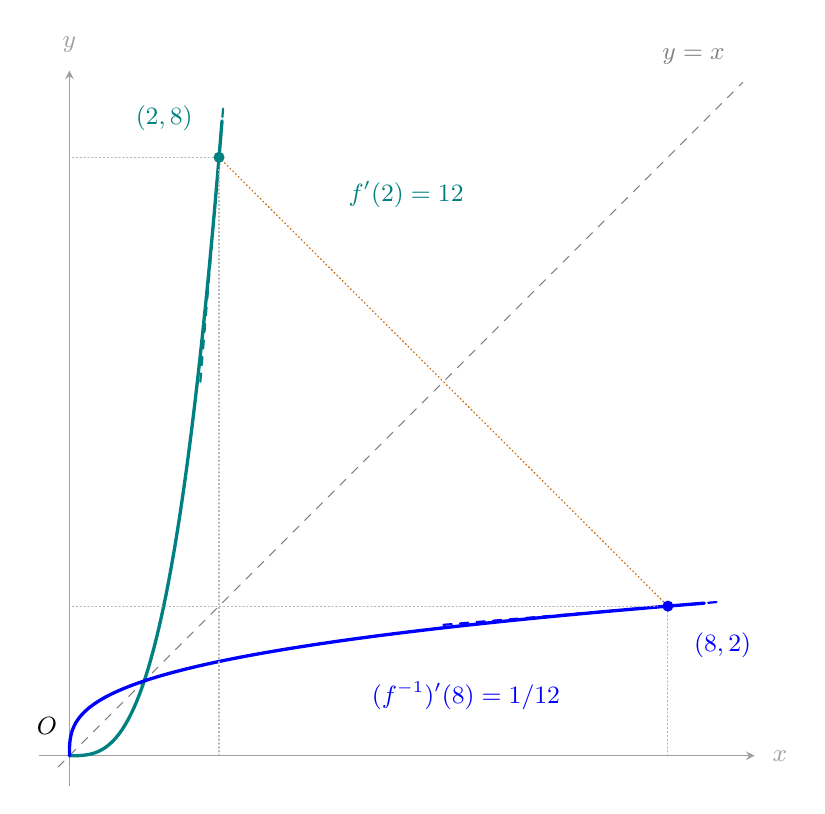
\begin{tikzpicture}[x=0.95cm,y=0.95cm,>=stealth,font=\small,line cap=round,line join=round]
\draw[->,gray!75] (-0.4,0)--(9.16,0) node[right=3pt]{$x$};
\draw[->,gray!75] (0,-0.4)--(0,9.16) node[above=3pt]{$y$};
\node at (-.3,.4) {$O$};
\draw[gray,dashed] (-0.15,-0.15)--(9,9) node[above left=3pt]{$y=x$};

\draw[teal,very thick,domain=0:2.04,samples=121] plot(\x,{\x^3});
\draw[blue,very thick,domain=0:2.04,samples=121] plot({\x^3},\x);
\draw[gray!60,densely dotted] (2,0)--(2,8)--(0,8) (8,0)--(8,2)--(0,2);
\draw[orange!80!black,densely dotted] (2,8)--(8,2);
\draw[teal,dashed,thick] (1.75,5)--(2.06,8.72);
\draw[blue,dashed,thick] (5,1.75)--(8.72,2.06);
\fill[teal] (2,8) circle(2pt) node[above left=6pt]{$(2,8)$};
\fill[blue] (8,2) circle(2pt) node[below right=6pt]{$(8,2)$};
\node[teal] at (4.5,7.5) {$f'(2)=12$};
\node[blue] at (5.3,.8) {$(f^{-1})'(8)=1/12$};

\end{tikzpicture}\par\smallskip
{\small \textcolor{teal}{\rule[.5ex]{1em}{.8pt}\ $y=x^3$}\qquad\textcolor{blue}{\rule[.5ex]{1em}{.8pt}\ $y=\sqrt[3]{x}$}}\par
{\small 先配对原函数上的点 $(2,8)$ 与镜像点 $(8,2)$，再取切线斜率的倒数。}\par\smallskip
\end{minipage}
\end{center}


设 $f(x)=x^3$，求其反函数在 $x=8$ 处的导数。

\textbf{解：}先找原函数对应输入：$a^3=8$，所以 $a=2$。原函数导数 $f'(x)=3x^2$，$f'(2)=12\ne0$。原函数连续严格递增，反函数连续，故
\[
\boxed{(f^{-1})'(8)=1/f'(2)=1/12}.
\]
不要把 $8$ 直接代入原函数导数。
\end{examplebox}
